%!TEX root = ../paper.tex

\subsubsection{Speeding Up Web Page Load} \label{label:whatif}

\begin{figure}
    \begin{subfigure}[b]{0.5\textwidth}
        \centering
        \includegraphics[width=1\linewidth]{sections/device-work/dsp-plt}
        \caption{Javascript execution (left axis) and emulated page load times (right axis)}
    \end{subfigure}

    \begin{subfigure}[b]{0.5\textwidth}
        \centering
        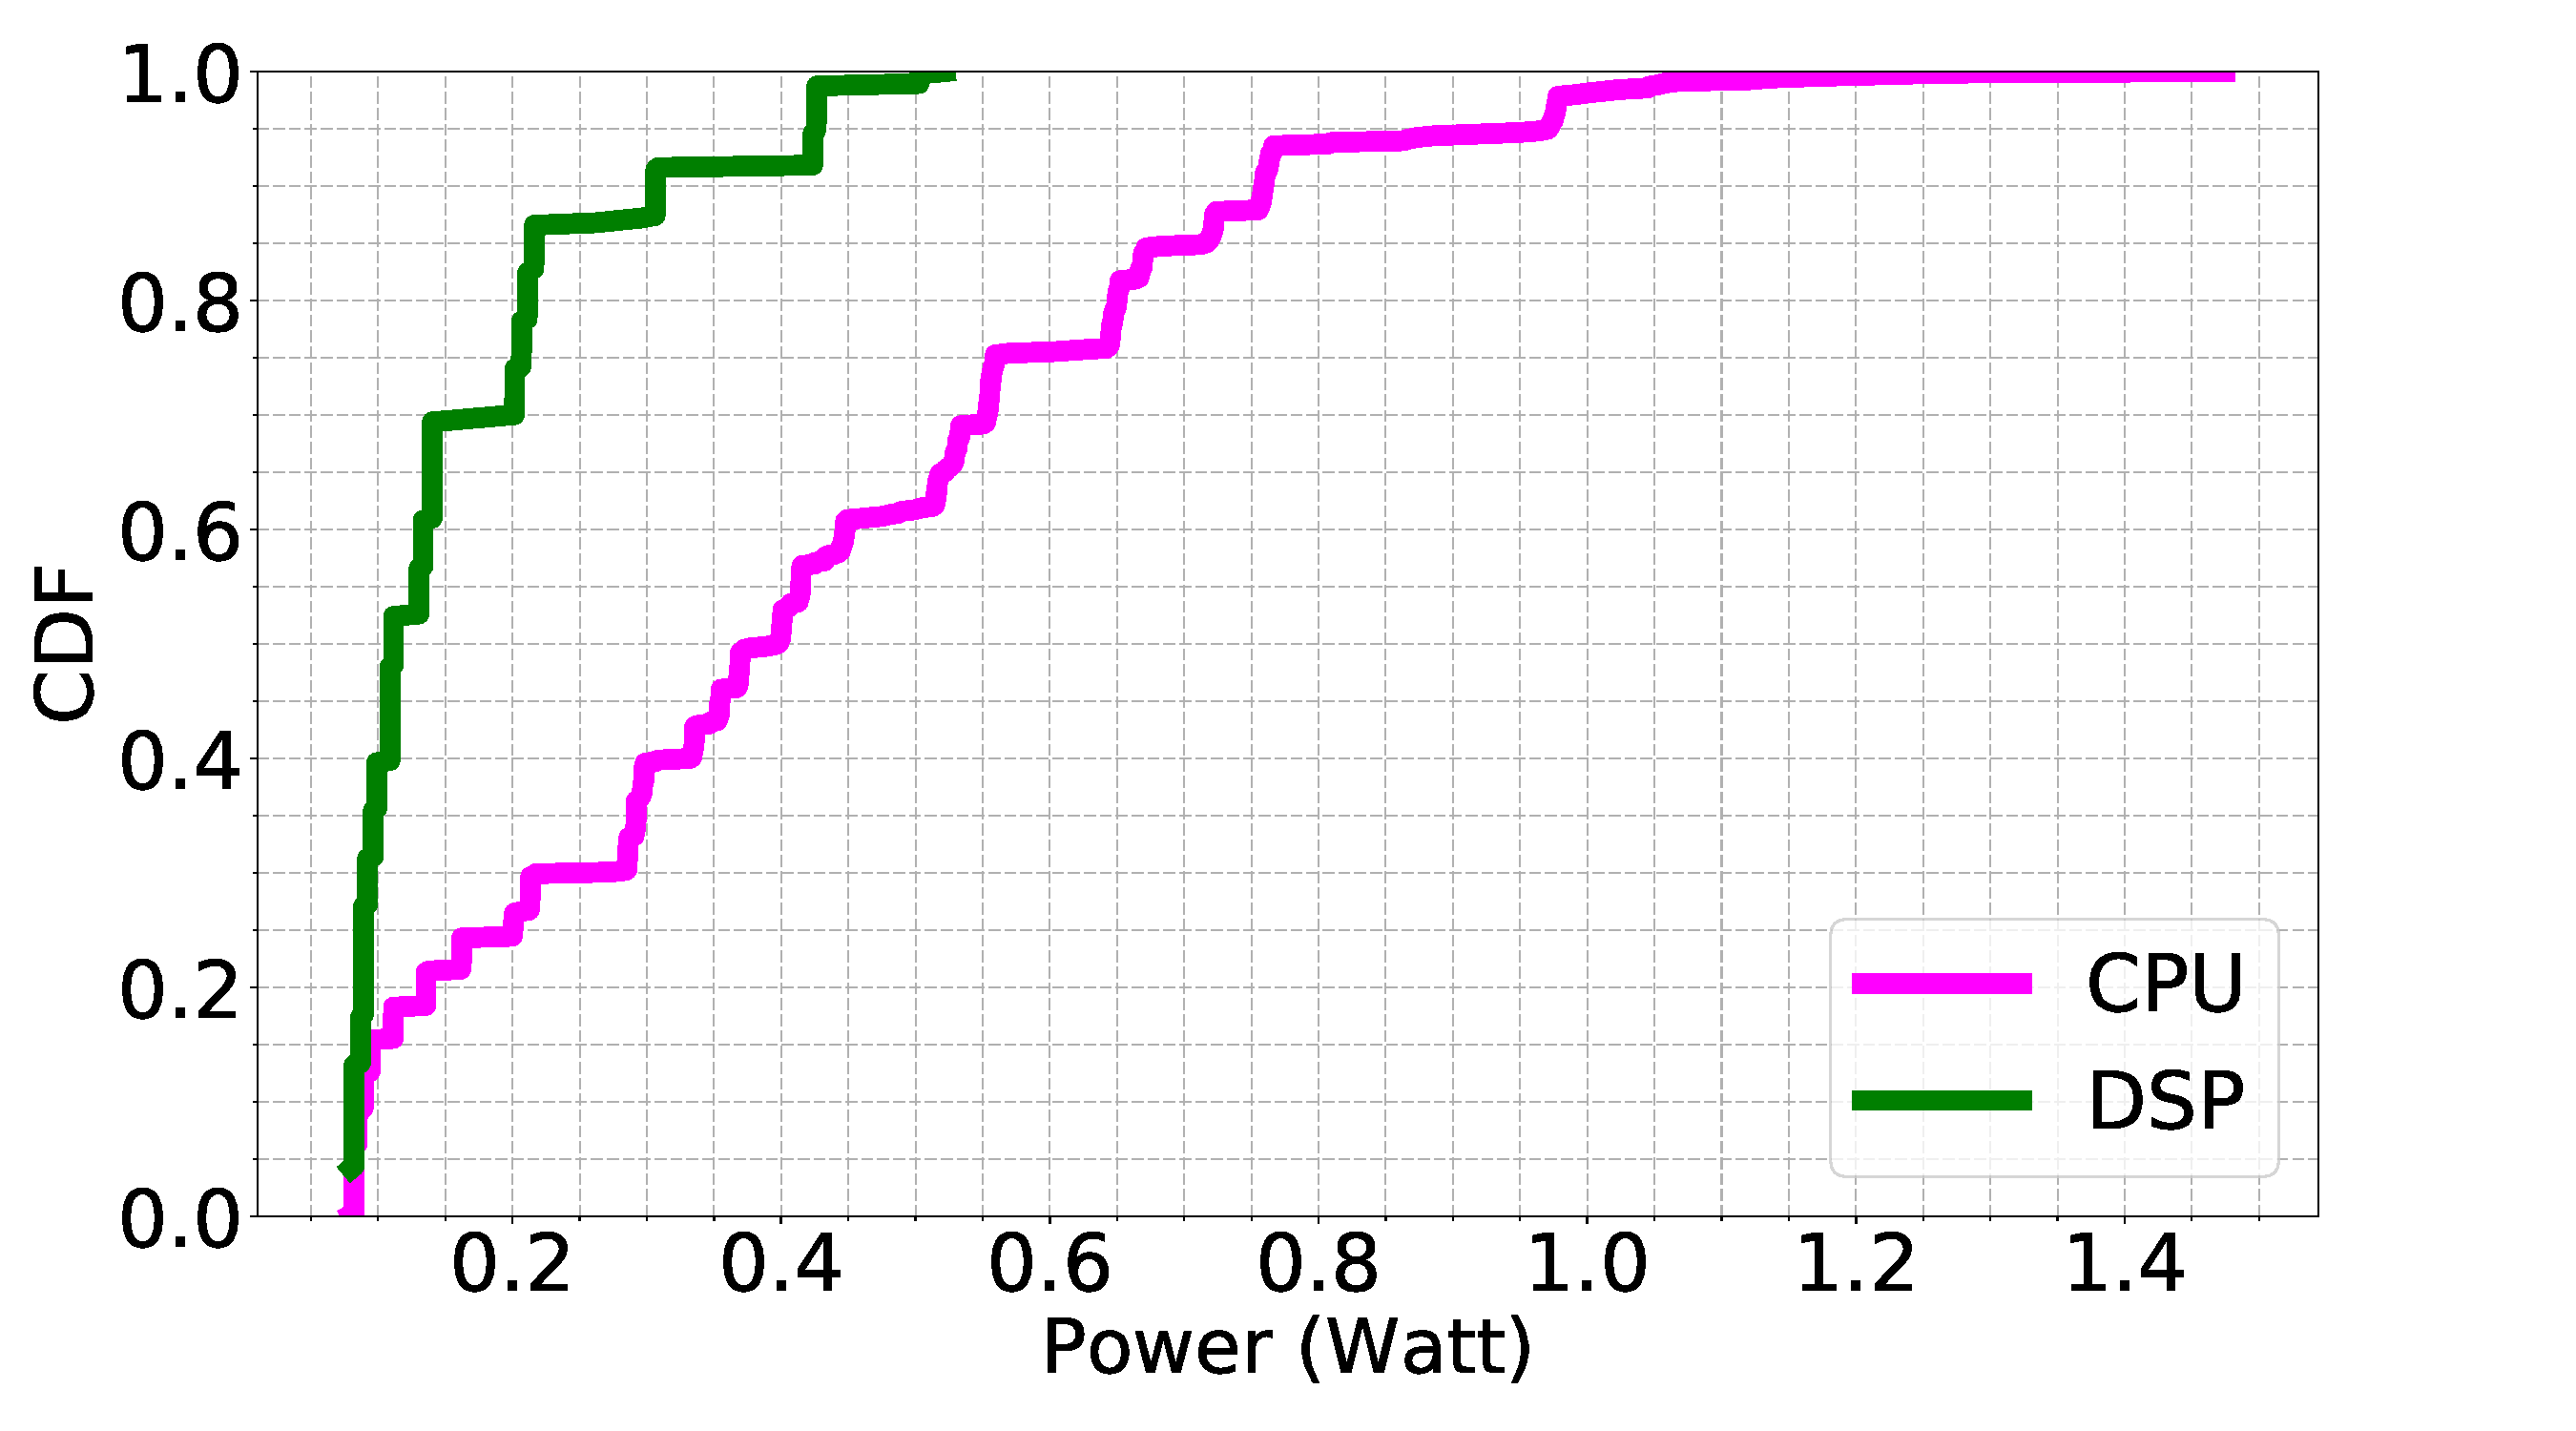
\includegraphics[width=1\linewidth]{sections/device-work/dsp-power}
        \caption{CDF of power consumption during Javascript execution}
    \end{subfigure}%

    \begin{subfigure}[b]{0.5\textwidth}
        \centering
        \includegraphics[width=1\linewidth]{sections/device-work/dsp-plt5}
        \caption{Emulated page load times with and without DSP offloading at low CPU frequencies}
    \end{subfigure}
   	\caption{Evaluations for DSP offloading of Javascript functions}
     \label{fig:dsp}
\end{figure}

%\begin{figure}[h]
%\begin{center}
%     \subfloat[Javascript execution (left axis) and emulated page load times (right axis) ]{%
%       \includegraphics[width=0.8\linewidth]{sections/dsp-plt}
%     }
% \end{center}
% \begin{center}    
%     \subfloat[CDF of power consumption during Javascript execution ]{%
%       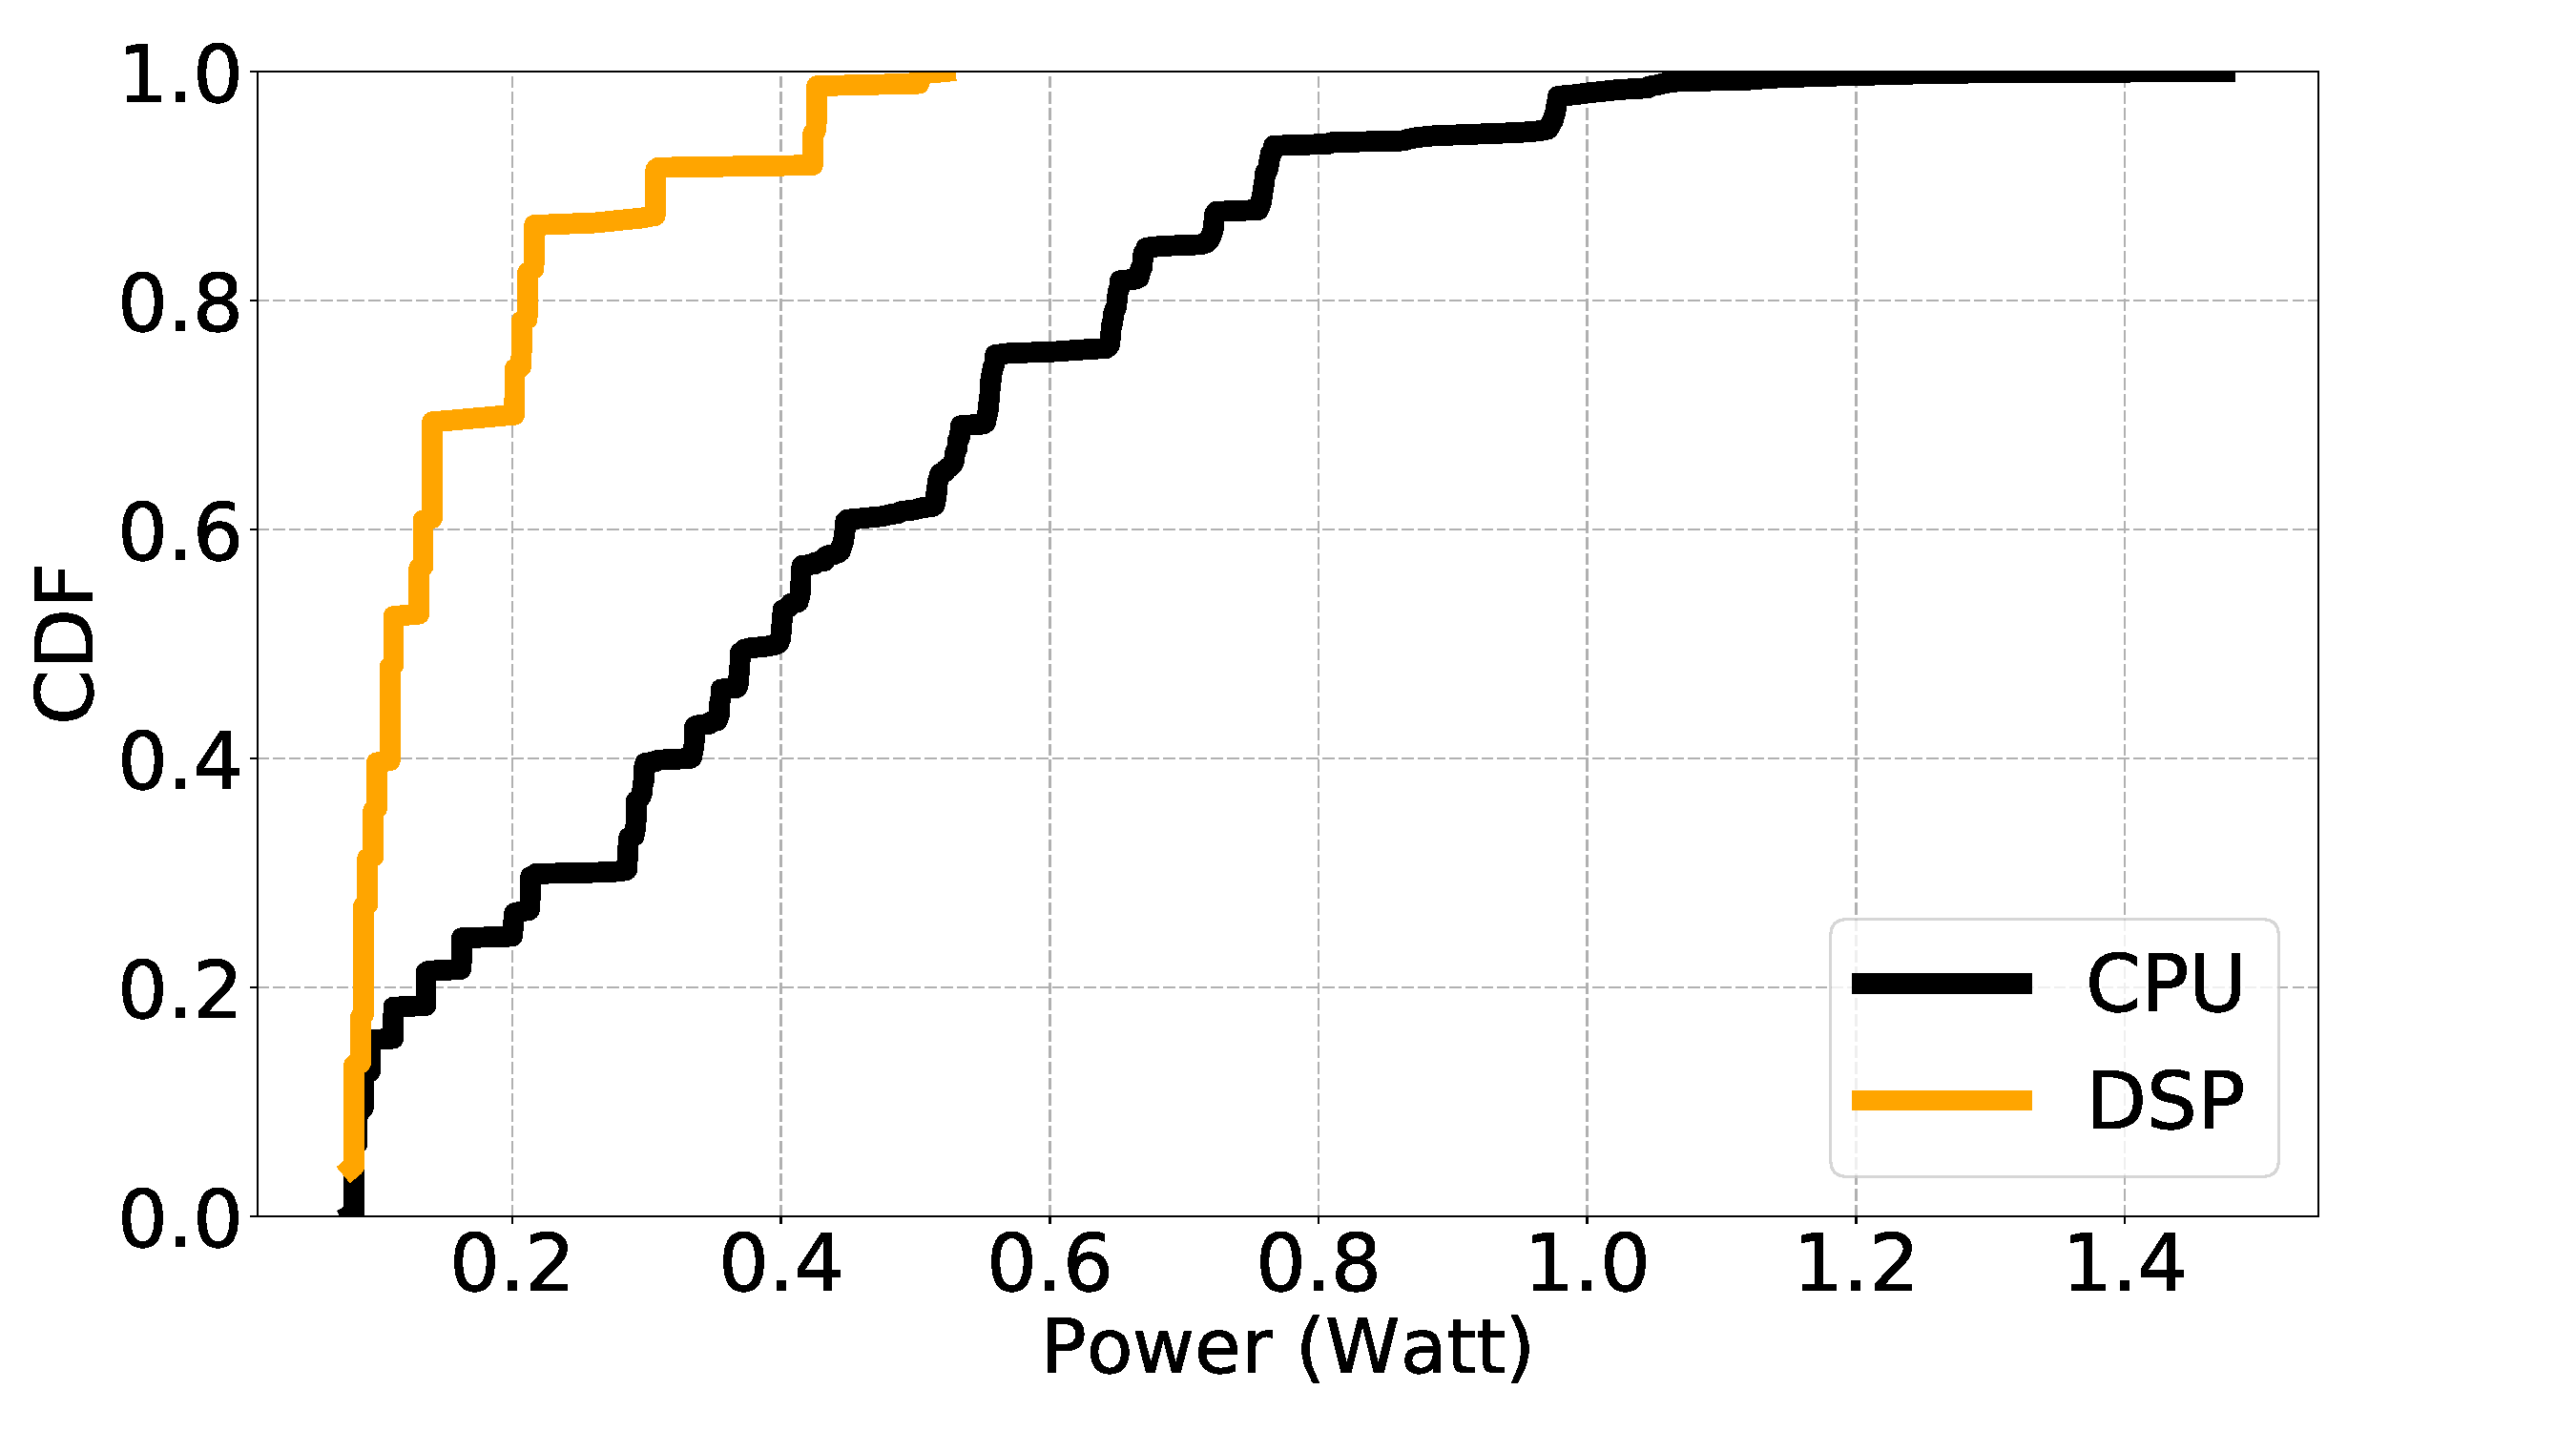
\includegraphics[width=0.8\linewidth]{sections/dsp-power}
%     }
%     \end{center}
%      \begin{center}    
%     \subfloat[Emulated page load times with and without DSP offloading at low CPU frequencies]{%
%       \includegraphics[width=0.8\linewidth]{sections/dsp-plt5}
%     }
%     \end{center}
%
%   	\caption{Evaluations for DSP offloading of Javascript functions}
%     \label{fig:dsp}
%\end{figure}

We learnt from our Web experiments (\S\ref{label:web}) that 
CPU frequency impacts web browsing performance more
than the other applications considered. This is a concern
for low-end phones as browsing performance
disproportionately suffers on these platforms. Video applications, on the other hand, are not severely impacted by CPU speeds because they offload compute to hardware. 

In this section, we conduct a {\em what-if} analysis to explore if offloading compute to a co-processor can also improve performance of Web page loads under low clock frequencies. Many mobile applications exploit co-processors like GPU and DSP and other specialized hardware accelerators. These co-processors provide faster processing and lower energy consumption if used effectively for appropriate
tasks (e.g., data parallel computing
for GPUs or floating point operations for DSPs.)
%So, it is 
%be interesting to explore whether browsing performance
%could improve by exploiting existing co-processors
%on the phone that otherwise would remain idle during
%typical browsing. The idea is to explore
%offloading computations to these co-processor(s)
%during the Web page load. 
 
%In this section, we discuss feasible approaches in improving the web browsing performance and their implications. We look at the following two approaches: 

%\begin{figure*}[t]
%       \centering
%       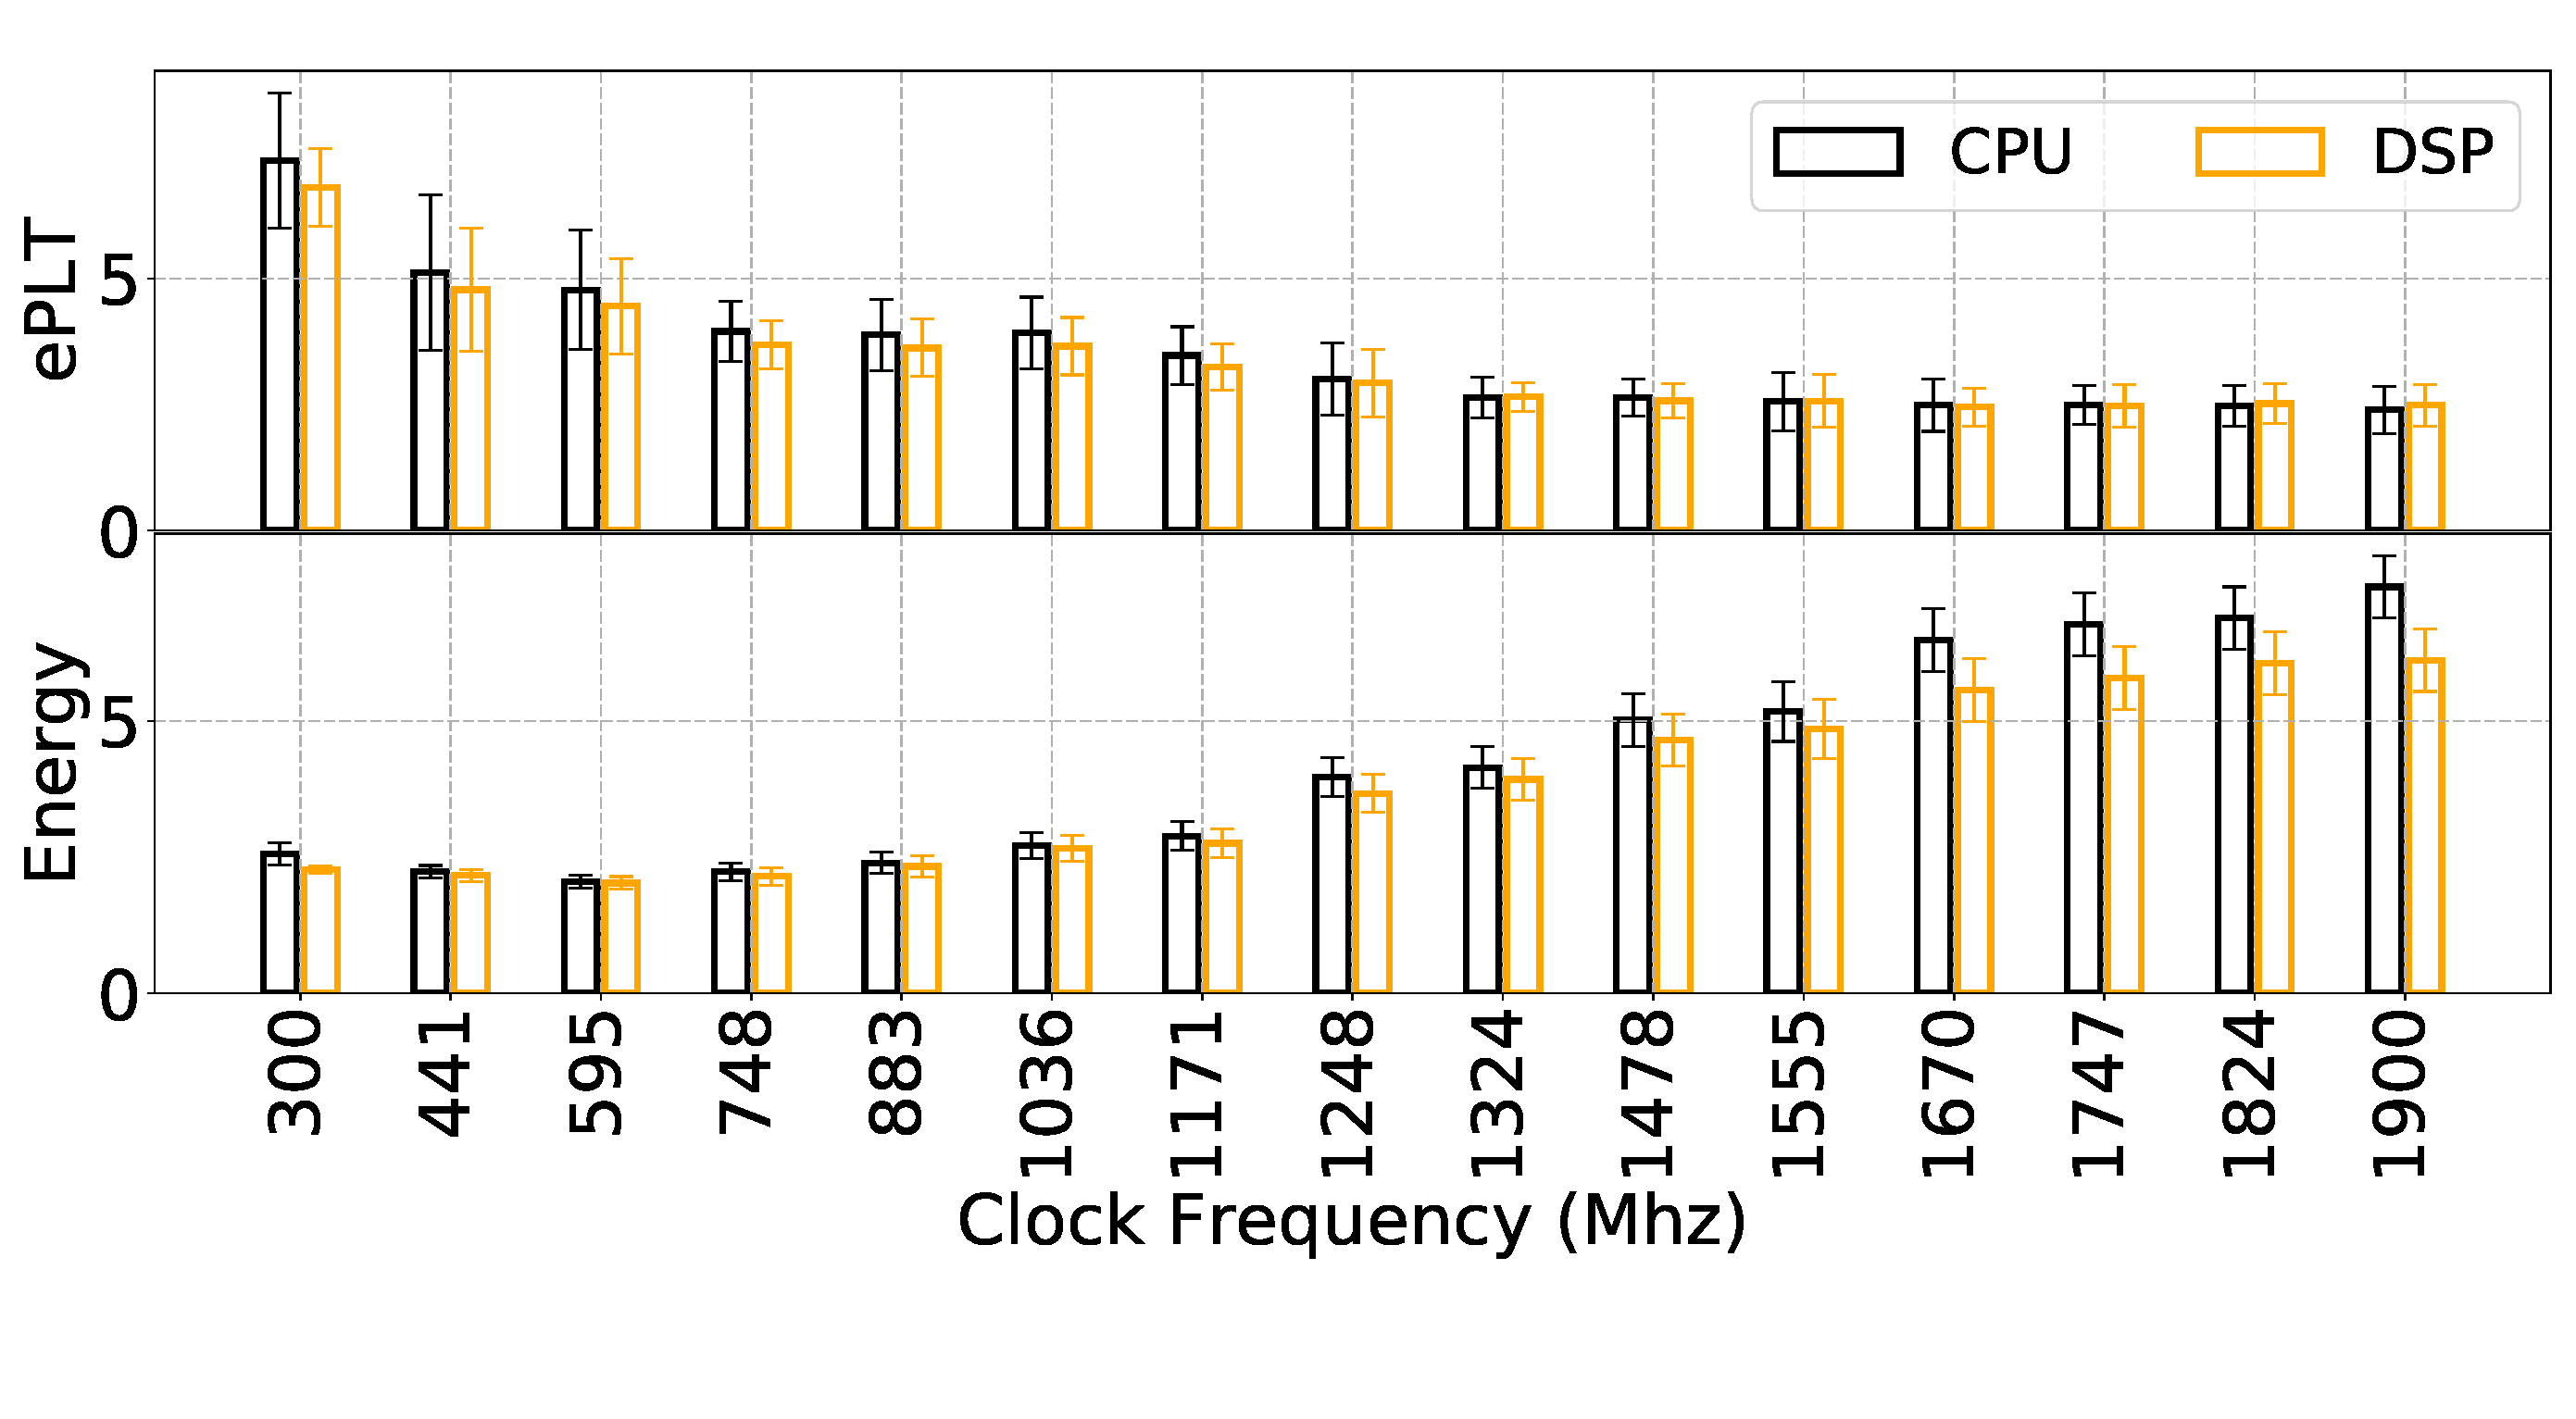
\includegraphics[width=\linewidth]{sections/dsp}
%       \caption{\textit{Emulated Page loads with DSP offloading under different CPU clock frequencies and Energy consumption with CPU and DSP}}
%       \label{fig:cpu-dsp}
%\end{figure*}



%\subsection{Use of Co-Processors:}

 %For example, GPUs demand massive data parallelism for faster processing and provide minimal energy consumption if all the GPU cores are used effectively. DSPs demand processing of complex multiplication instructions so it can pack all the work in a single instruction executed in a single pipelined execution \cite{codrescu2014hexagon}. 
To this end, we systematically look at computations during
Web page load. Scripting/Javascript execution is the most
time-consuming computation (Figure~\ref{fig:dissect}). By manually
evaluating scripting functions
for the slowest set of Web page loads in our experience, i.e., the sports
pages (Figure~\ref{fig:sites-effect}), we find 
that a significant time is spent in regular 
expression (regex) evaluations (e.g., for 
URL matching, list operations). Our goal is to explore offloading the regular expression evaluation to the DSP. GPU is not appropriate as these computations are not data parallel.

The following paragraphs describe the experiments
and the evaluations leading to 
plots in Figure~\ref{fig:dsp}. In summary,
offloading the regex part of Javascript 
execution to the DSP provides a modest
improvement in estimated PLT when the mobile device is run with default frequency governors, where the CPU frequency is set by the OS (Figure~\ref{fig:dsp}a). 
A significant improvement is, however, noticed
in the power consumption -- almost $4\times$ reduction
in median power consumption (Figure~\ref{fig:dsp}b). The PLT improvements are larger (up to 25\%) when the Web page is loaded under slower CPU speeds (Figure~\ref{fig:dsp}c). While
not completely conclusive, these evaluations show that 
offloading of the compute intensive part of Web browsing 
to co-processors does have potential
and should be explored. 

%As we observe a lot of computation bottlenecks in mobile webpage loags, we investigate the feasibility of offloading this computation onto these co-processors. Parsing and Scripting are the two main bottlenecks that constitute upto 40\% (\S\ref{label:web}) of total PLT. Parsing is a step by step instruction fetch, decode and execute procedure which is neither data parallel nor has complex instructions, therefore not suitable for either of the co-processors. However, we observe a potential for scripting functions (such as regex processing in URL matching, list operations) to offload onto these co-processors. While this computation is not highly data parallel, these complex instructions can be offloaded to DSPs.

%\todo{This text below is too tedious. Not sure whether we should move this to an appendix.}

\noindent\textbf{Details of Evaluation:}
We use Qualcomm Hexagon SDK \cite{hexqual2013qcom} to offload Javascript functions to the DSP.
As the SDK is limited to low-level languages such as C/C++, it is not straight-forward to port Javascript code to the DSP.
%At the same time, offloading entire javascript is also not a good idea because of the entire processing is not suitable for DSPs.
Instead, we extract regex functions from the Javascript
and convert them to C-language libraries. %We load them in Javascript functions 
%using SWIG library \cite{swigcjs}.

%We use this compute performance and replay only object downloads to emulate page load. We call this as \textit{ePLT}. 
%For this reason we cannot directly evaluate PLT.
We then port the converted C code onto the \textit{aDSP} processor on a Google Pixel\,2 phone
(which has the Snapdragon 835 Application processor). 
The Inter Process Communication (IPC) between CPU and DSP takes place through 
the FastRPC remote procedure call.

Since the offloading cannot be directly performed on the browser, we use nodejs to run these functions to evaluate their runtime performance. In effect, we record the page load process and extract the dependency graph with WProf~\cite{wang2013demystifying}. WProf preserves the dependency and computation timing information during the page load. For each Javascript evaluation that contains regex, we estimate the time taken if the regex evaluation were offloaded. Based on this new timing, we re-evaluate the dependency graph and compute the new page load time that we call emulated PLT or ePLT. We experiment on the top 20 sports Web pages.

%We run these experiements on Google Pixel2 phone which comes with Qualcomm Snapdragon 835 Application processor. This processor comes with two DSP processors: \textit{mDSP} and \textit{aDSP}. mDSP is standalone processor for modem functionality, while aDSP is used for customized applications.

 %The CPU calls a remote mothod on the DSP and sleeps until DSP updates its status. 
%Here, the input/output buffers are transferred to DSP in the form of arguments to the remote method which is an expensive operation. This becomes the main bottleneck if we offload shorter processing blocks onto DSP. However, the inherent ability of DSP to achieve ultra low power processing makes it more promising to offload even such minimal computation.

%\noindent\textbf{Evaluation:} 


% show results for the Javascript execution, ePLT and power consumption for
%two cases i) regular execution on CPU, ii) regex executions offloaded to DSP. 
%There is about 18\% \todo{ check} improvement in the script execution times
%and ePLT. While this is modest, the improvement in power consumption is substantial - about $4\times$. 
%While these experiments are done on a high-end phone using the default frequency
%governor separate experiments (not shown for brevity) demonstrate that these experiences
%translate well to the scenario when the clock is slow. 
%We run this experiment under all CPU clock frequencies for 20 runs. Note that, we experimented with only available clock frequencies on Pixel2.

%Figure \ref{fig:cpu-dsp} shows ePLT for CPU and DSP for all clock frequencies.
%We observe an improvement of 0.5 to 1second on average ePLT under DSP until 1248Mhz clock, then equal performance till 1747Mhz and less than 100ms under higher clock frequency. 
%This descrepancy is due to two reasons: First, IPC overheads such as memory buffer transfers incurrs latency which is making the ePLT bad under higher clock where the CPU performs best. Second, the offloaded computation is very short ($<1.5$ seconds) which is less than 20\% overall ePLT.
%Although the ePLT improvement is a little, we observe very low energy consumption under DSP, as it is specifically designed to be power efficient. 
%Figure \ref{fig:cpu-dsp} shows that DSP consumes less energy than CPU always and performs better especially under higher clock. There is a consistent reduction of 2 Joules from 1670Mhz to 1900Mhz clock.
%This shows that instead of overclocking the phone to improve the performance, DSP coprocessor helps improve the performance as well as energy under lower clocks.

%We also run this experiment under default settings i.e., without fixing a clock frequency.
% Figure \ref{fig:dsp} shows the emulated pageloads and scripting time under DSP and CPU under default settings. 
% The pure scripting time on DSP without these overheads (DSP W/O) shows an improvement over 100ms. 
% The scripting with IPC overheads shows that both CPU and DSP show almost same (55ms) of scripting time. 
% The emulated pageloads corresponding to these script times are shown on green axis. 
% The \textit{ePLT} is again almost same (~4seconds) with CPU and DSP. 

% We aslo observe energy consumption under default settings. 
% Figure \ref{fig:dsp} (b) shows that DSP consumes less than 400mW of power consistently for scripting, while CPU is taking upto 1.4Watts of power. 
% Therefore, DSP offloading of computation certainly helps performance as well as energy improvements. 

%\subsection{DOM Parallelization}
%The Document Object Model (DOM) is a logical structure that represents webpage elements including HTML content, element relationships, visual styles and the positions of each element. HTML, Javascript, and CSS manipulate the DOM in producing the final webpage footprint. Most of the current browsers impose restrictions on accessing DOM in a serial manner. As a result, these page processing tasks are heavily dependent upon each other, resulting in blocking and underutilization of compute resources. Our hypothesis is that speculative parsing of HTML and parallelization of JavaScript execution has the potential to decrease the overall PLT of a webpage by fully utilizing device compute power. \\
%\textbf{Implementation:} We use our emulator, \textit{PALO} which is short for \textit{Page Loader}, to evaluate the PLT under a DOM-parallelized scenario. The set-up of \textit{PALO} for emulating the parallelization of computation activities is similar to the setup described in \S \ref{label:web}. However, \textit{PALO} is able to replay the dependency events by emulating the computation activities in parallel. Specifically, direct dependencies are replayed in parallel with their parent activities while timed dependencies must still wait for the parent activities to schedule them. Furthermore, we also emulate a scale-up in the processor compute power to observe the impact of a higher clock frequency in comparison to parallelization. \\
%\textbf{Evaluation:} Fig. \ref{fig:dom-par} shows \textit{ePLT} under parallelized DOM access for scripting and parsing. It shows that with best possible parallization, the \textit{ePLT} improvement is 4.5 seconds over default \textit{ePLT}. With parallelization and scale-up together, the improvement is 5 seconds. Further, the compute power scale-up (double) alone shows a minimal ($<$2 seconds) decrease in \textit{ePLT}. This shows that parallelization helps a lot compared to compute power. However, the DOM parallelization is not a practical solution and must be serialized to conform to HTML5 specification \cite{html5spec}.
%\begin{figure}[t]
%   \centering
%   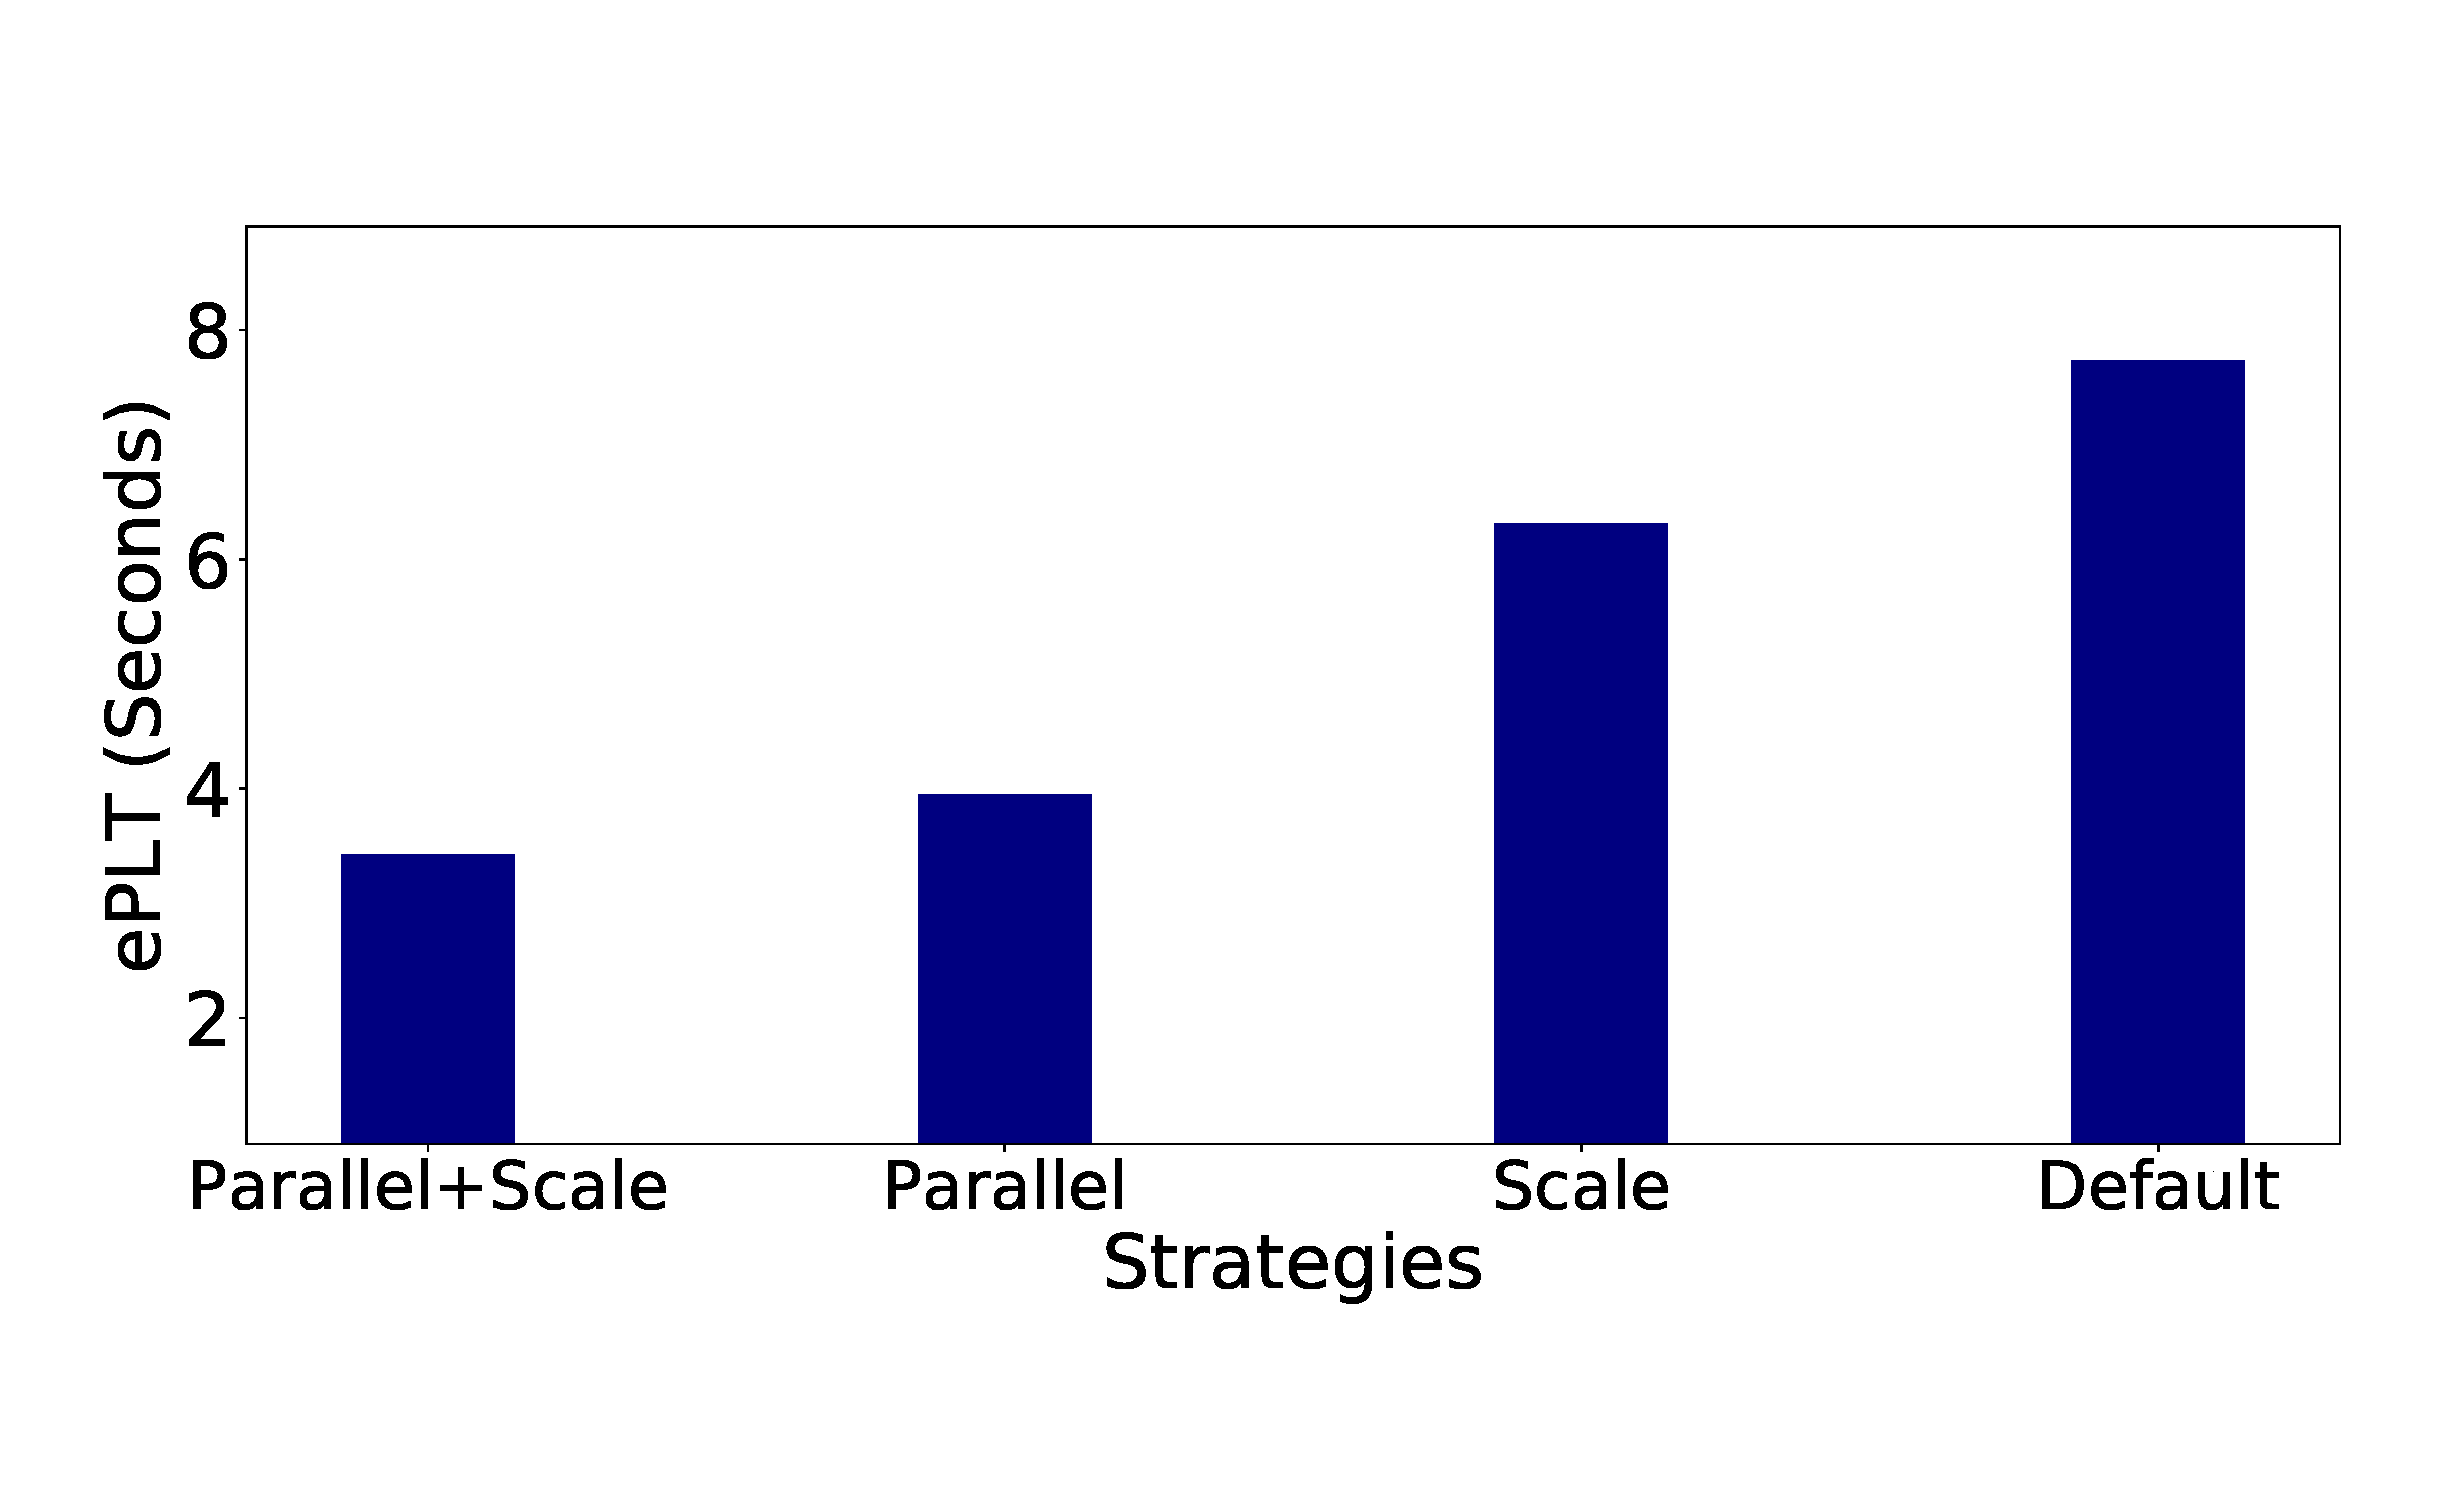
\includegraphics[width=\linewidth]{sections/dom-par}
%   \caption{\textit{Emulated Page loads under DOM Parallelization and Scaling the compute power.}}
%   \label{fig:dom-par}
%\end{figure}
